
\documentclass[12pt]{report}
\usepackage[backref=page]{hyperref}
\usepackage{listings}
\usepackage{multirow}
\usepackage{adjustbox}
\usepackage{graphicx}
\graphicspath{{images/}}

\hypersetup{
    colorlinks=true,
    linkcolor=black,
    filecolor=magenta,
    urlcolor=cyan,
    citecolor=blue,
    pdftitle={Design Document},
    pdfpagemode=FullScreen,
}

\lstset{
    basicstyle=\footnotesize\ttfamily,
    columns=fullflexible,
    frame=single,
}

\author{Stefan-Nikola}
\title{Design Document (CloudCord)}
\date{2024}

\begin{document}

\maketitle

\tableofcontents

\chapter{Introduction} 

The idea of my project is a microservice-based Discord-like clone named CloudCord. The idea is to utilize best practices and the cloud to get reliable, maintainable and scalable communication platform to connect people from everywhere.

\section{Scope} 

The scope of this project is to have a simplistic communication platform that takes advantage of cloud best practices. 

\chapter{Requirements} 

\section{Functional requirements} 

\begin{enumerate}

    \item The platform must implement a secure authentication mechanism that supports industry-standard authentication protocols.

    \item The platform must include a comprehensive monitoring to track application performance, security events, and system health.

    \item The platform must utilize Kubernetes for container orchestration, enabling dynamic scaling of microservices. 
  
    \item The platform must integrate a Continuous Integration/Continuous Deployment (CI/CD) pipeline to automate code testing, building, and deployment. 

\end{enumerate}

\section{Non-functional requirements} 

\begin{enumerate}

  \item \textbf{Fault Tolerance:} The system should follow best practices for microservices architecture to ensure that the failure of one service has minimal impact on the rest of the platform.

   \item \textbf{Security:} User data should be securely stored and transmitted to prevent unauthorized access. 

\item \textbf{Scalability:} If a service's resource usage exceeds 50\% for at least 1 minute, the system should automatically scale resources to maintain performance during peak usage.

\item \textbf{Performance:} The system should respond to user requests within 2 seconds under normal load conditions.

\item \textbf{Testing:} The system should run automated tests for every code change in the CI/CD pipeline to ensure functionality and stability before deployment.

\end{enumerate}

\chapter{Design details} 

\section{Backend (Golang) - High-Performance Microservices}

\textbf{Design Overview:} The backend will consist of a series of high-performance microservices developed in Go. Go is chosen due to its concurrency model, speed, and simplicity. Each microservice will be responsible for a specific domain (e.g., user authentication, messaging, notifications, etc.). These services will interact through REST APIs and gRPC for internal communication, ensuring low latency and high throughput.

\textbf{Service Design:}
\begin{itemize}
    \item \textbf{User Service:} Handles user-related information such as registration, authentication, and user preferences.
    \item \textbf{Chat Service:} Responsible for sending and receiving messages between users, including text-based communication.
    \item \textbf{Voice Service:} Manages voice communication between users using WebRTC for real-time voice interaction.
    \item \textbf{Notification Service:} Sends notifications (e.g., when a message is received or when a user is mentioned).
    \item \textbf{File Storage:} Stores unstructured data such as files, images, and other media content.
\end{itemize}

\textbf{Communication:} Microservices will communicate through RESTful APIs for external communication and asynchronous messaging via message queues for internal communication. This ensures decoupling of services and enables efficient event-driven processing.

\textbf{Scalability:} Each service can scale independently based on demand, using Kubernetes for orchestration and Docker for containerization. This allows for flexible scaling of individual services depending on the traffic and load they are handling.
 provide documentation that explains all the code and how everything works, together with examples and API references. 

\section{Frontend (React) - Modern, Responsive UI}

\textbf{Design Overview:} The frontend will be developed using React to provide a modern and responsive UI. React's component-based architecture will ensure that the user interface is dynamic and can efficiently update as state changes.

\textbf{Key Features:}
\begin{itemize}
    \item \textbf{Real-time Chat Interface:} For text-based communication between users, allowing users to send and receive messages in real-time.
    \item \textbf{Voice Call Interface:} For managing voice and video communication using WebRTC, providing a seamless experience for voice and video calls.
    \item \textbf{Sidebar:} Displays server lists, chat channels, and friends, allowing users to quickly navigate between different areas.
    \item \textbf{Notification Area:} Shows incoming messages, mentions, or other notifications, ensuring users are promptly alerted.
\end{itemize}

\textbf{Communication:} WebSocket connections will be used to facilitate real-time messaging, ensuring low-latency communication between users for both chat and voice/video features. This will enable a seamless, interactive experience with instant updates.



\section{WebSockets \& WebRTC - Real-time Messaging \& Voice/Video}

\textbf{WebSockets:} WebSockets will be used for real-time, bidirectional communication between the client and server. This allows users to send and receive messages instantly without needing to refresh the page. The backend will handle the WebSocket connections for chat services and notifications.

\textbf{WebRTC:} WebRTC will be implemented for peer-to-peer voice and video communication. WebRTC is efficient and allows low-latency media transfer, which is crucial for a communication platform.

\textbf{Design:}
\begin{itemize}
    \item WebSockets will be initiated on the frontend (React) and managed by the backend through a WebSocket server built with Go.
    \item WebRTC sessions will be handled via signaling between the client (React) and a signaling server built with Go. This will enable real-time communication setup for voice and video calls.
\end{itemize}


\section{Database (PostgreSQL \& MongoDB) - Relational Storage + Unstructured Storage}

\textbf{PostgreSQL:}
\begin{itemize}
    \item \textbf{Usage:} This will be used for structured, relational data, such as user profiles, channel memberships, permissions, and message histories.
    \item \textbf{Design:} Tables for users, channels, messages, and server roles.
    \item \textbf{Scalability:} PostgreSQL can be scaled vertically (by improving hardware) or horizontally using replication.
\end{itemize}

\textbf{MongoDB:}
\begin{itemize}
    \item \textbf{Usage:} This will handle unstructured or semi-structured data, such as message content (if large attachments or logs need to be stored), real-time chat logs, and user metadata (preferences, settings).
    \item \textbf{Design:} Collections for messages, user settings, etc., allowing flexible schemas.
    \item \textbf{Scalability:} MongoDB provides horizontal scalability through sharding, ensuring that data grows without degrading performance.
\end{itemize}

\section{Containerization and Cloud Deployment (Kubernetes \& Docker) - Scalable Infrastructure}

\textbf{Docker:}
\begin{itemize}
    \item \textbf{Usage:} Each microservice will be containerized using Docker to provide an isolated, reproducible environment for the service.
    \item \textbf{Design:} Each service (e.g., User Service, Messaging Service) will have its own Docker image and a Dockerfile that specifies dependencies, build steps, and runtime configuration.
\end{itemize}

\textbf{Kubernetes:}
\begin{itemize}
    \item \textbf{Usage:} Kubernetes will be used for orchestrating containers, ensuring that the system is highly available, fault-tolerant, and scalable.
    \item \textbf{Design:}
    \begin{itemize}
        \item Kubernetes will manage service discovery, load balancing, scaling, and resource management (CPU, memory).
        \item Helm charts will be used for deploying services with Kubernetes, ensuring easy updates and management.
        \item Auto-scaling will be enabled to dynamically scale services based on resource usage.
    \end{itemize}
\end{itemize}
 
\section{CI/CD - Automated Testing and Deployment}

\textbf{CI/CD Pipeline:} The CI/CD pipeline will automate the testing, building, and deployment processes.

\textbf{Tools:}
\begin{itemize}
    \item \textbf{CI:} GitHub Actions or Jenkins for continuous integration, triggering tests on code commits.
    \item \textbf{CD:} ArgoCD or Helm for continuous deployment, pushing updates to the Kubernetes cluster automatically after tests pass.
\end{itemize}

\textbf{Design:}
\begin{itemize}
    \item On each commit, the code will be tested (unit tests, integration tests).
    \item If tests pass, the Docker containers will be built and pushed to a container registry (e.g., Docker Hub, ECR).
    \item Kubernetes will pull the updated containers, ensuring that the latest version of the app is deployed.
\end{itemize}

\textbf{Testing:}
\begin{itemize}
    \item Automated tests (unit, integration, performance tests) will be integrated into the pipeline to ensure the reliability of each change.
    \item \textbf{Quality Gate:} Only code passing tests will be allowed to move to production.
\end{itemize}
 

\section{Monitoring (Prometheus + Grafana) - Live Metrics and Health Tracking}

\textbf{Prometheus:}
\begin{itemize}
    \item \textbf{Usage:} Prometheus will be used to collect real-time metrics from microservices, such as CPU usage, memory usage, request latency, and error rates.
    \item \textbf{Design:} Each service will expose a \texttt{/metrics} endpoint, which Prometheus will scrape at regular intervals. This will provide insight into the health and performance of each service.
\end{itemize}

\textbf{Grafana:}
\begin{itemize}
    \item \textbf{Usage:} Grafana will be used for visualizing the data collected by Prometheus. Dashboards will show real-time health, performance, and system metrics (e.g., CPU usage, response times, request throughput).
    \item \textbf{Design:} Grafana will be integrated into the monitoring stack, providing real-time insights for the platform operators.
\end{itemize}

\textbf{Alerting:}
\begin{itemize}
    \item Prometheus will be configured to trigger alerts when metrics exceed predefined thresholds (e.g., high error rates, low availability). Alerts will be sent to Slack or email to notify the team of issues in the system.
\end{itemize}














\chapter{Architecture design} 

     \begin{figure}[htbp]
      \centering
        \adjustbox{max width=\textwidth, max height=\textheight}{
          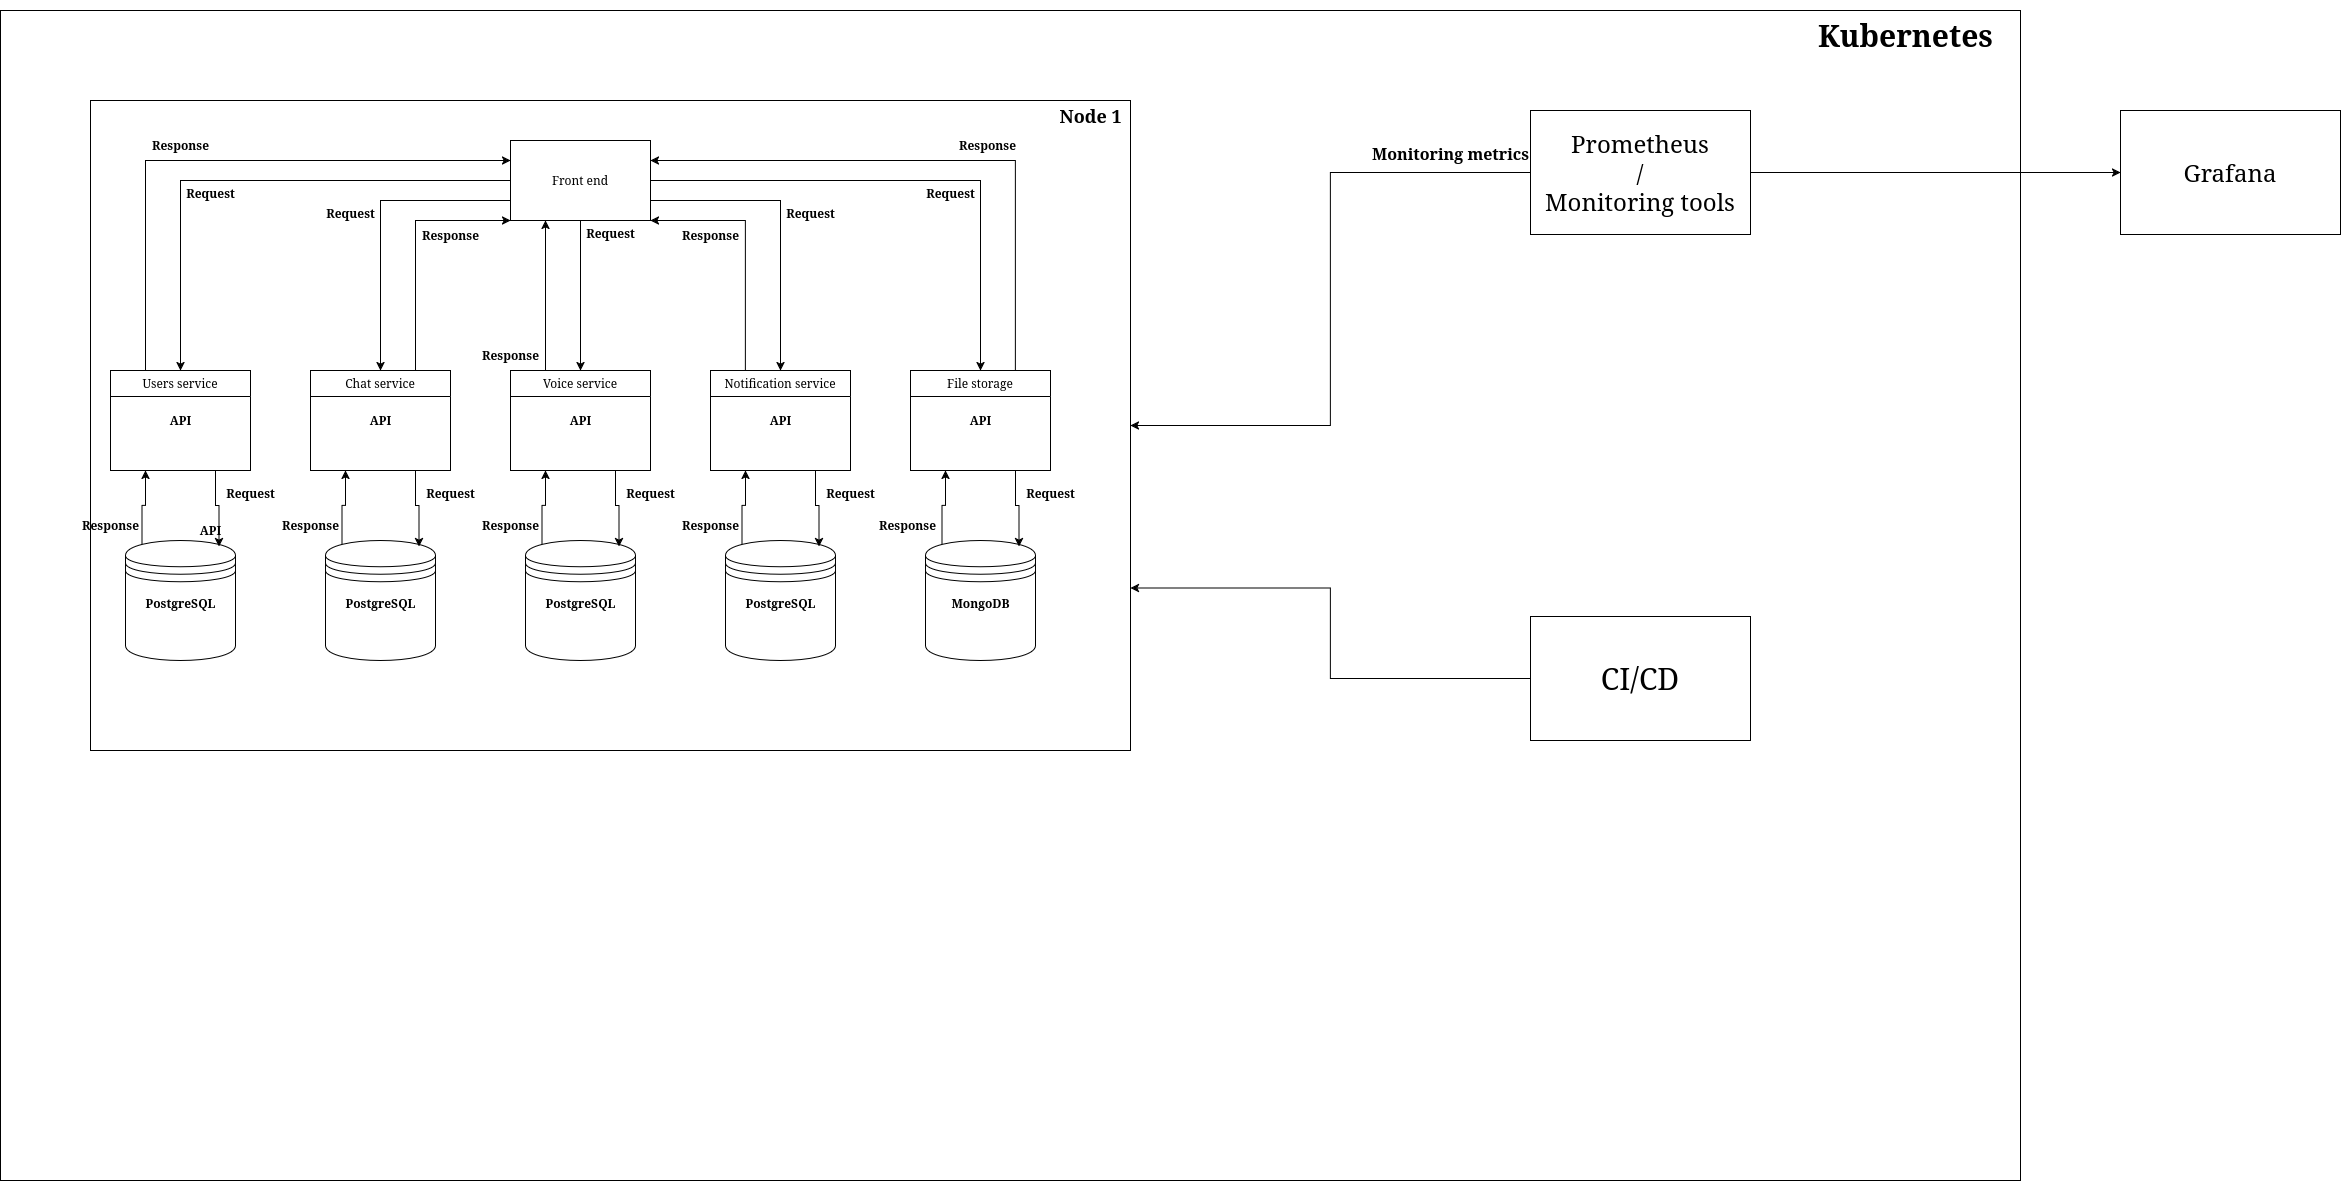
\includegraphics{Architecture.png}
      }
        \caption{Architecture design} 
    \end{figure}   

\chapter{Testing} 

\begin{enumerate}

    \item[]For testing I'll conduct the following testing methods:

    \item CI/CD automation

      \item Unit testing 

      \item Integration testing 

      \item Manual testing 

\end{enumerate}

\end{document}
